\vspace*{-0.2cm}
\section{Experimental Evaluation}
\vspace*{\subsecspace}
\label{sec:eval}

% Run on system with Ubuntu, 48 phys cores, Nvidia P100 GPU, 250 Gb ram
% Here we will showcase the effectiveness of our GPU memory manipulation in minimizing
Here, we showcase the many parts of our design in an extensive series of experiments that fully analyze its impact.
All experiments were run on identical systems running Ubuntu 20.04 on kernel version 5.4, with a 48 physical core Intel Xeon Platinum 8160 with hyperthreading disabled, 250 GB of RAM, and an Nvidia P100 GPU running driver version 470.239.06.
This isn't the latest GPU hardware, and emphasizes that our design can work with a variety of hardware, doesn't require advanced features, and is easily scalable and adaptable to other systems.

\subsection{UVM Shim}
\label{sec:shim}

The piece underpinning our entire design is our driver shim that captures and rewrites memory allocations made by function code.
If we cannot oversubscribe memory or can only do so by significantly increasing code execution time, our system design is untenable.

\mhead{Memory Management}
Our shim enables two abilities, GPU memory overcommitment and control plane management of memory placement.
To show the impact of both we run 16 copies of the FFT function from Table~\ref{tab:fun-list}, each using 1.5 GB of device memory that, in aggregate, oversubscribes our GPU's memory by 50\%.
% To show the importance of locality of function memory and available space, we run 16 copies of the FFT function from Table~\ref{tab:fun-list}, each using 1.5 GB of device memory that, in aggregate, oversubscribe GPU memory by 50\%.
We then invoke them individually and iteratively 20 times such that all will be executed before starting executing the first again.
Before and after invocations, we direct our shim to prepare function memory in various ways.
The impact of these different memory policies are displayed in Figure~\ref{fig:mem-prefetch}, with average time spent in-shim shown in red and function code execution in black.
With such high oversubscription, UVM driver alone controlling data placement, the \texttt{None} case, execution time is 40\% worse than the optimal seen in Table~\ref{tab:gpu-cpu}.
Execution time is higher when memory must be paged in on-demand from the host as kernels access it, and old memory paged out.
% An intial proactive mechanism of telling the driver our data location preference, \texttt{Madvise}, tells the CUDA memory system we would prefer the memory onto the card, and after execution to prefer it off.
Using just the driver madvise mechanisms, \texttt{Madvise}, tells the CUDA memory system we would prefer memory on the card, and after execution to prefer it off.
This actually is worse than \texttt{None}, as madvise calls to the driver don't actually move any memory, we just waste time sending the memory directives with no benefit to execution time.
Active prefetching with \texttt{Prefetch To} asynchronously copies memory to the device before invocation, and \texttt{Prefetch} additionally moves data off device after execution.
If we only tell the driver to move memory \textit{onto} the device, it must spend time page swapping to fulfill our request, and potentially move pages we still need.
Combining removal of idle memory \emph{and} prefetching memory in anticipation of use reduces function latency by 33\% over \texttt{None}.
We send prefetching directives off the critical execution path, thereby reducing the latency to just execution time, which now matches the ideal execution time as listed in Table~\ref{tab:gpu-cpu}.

\begin{figure}
  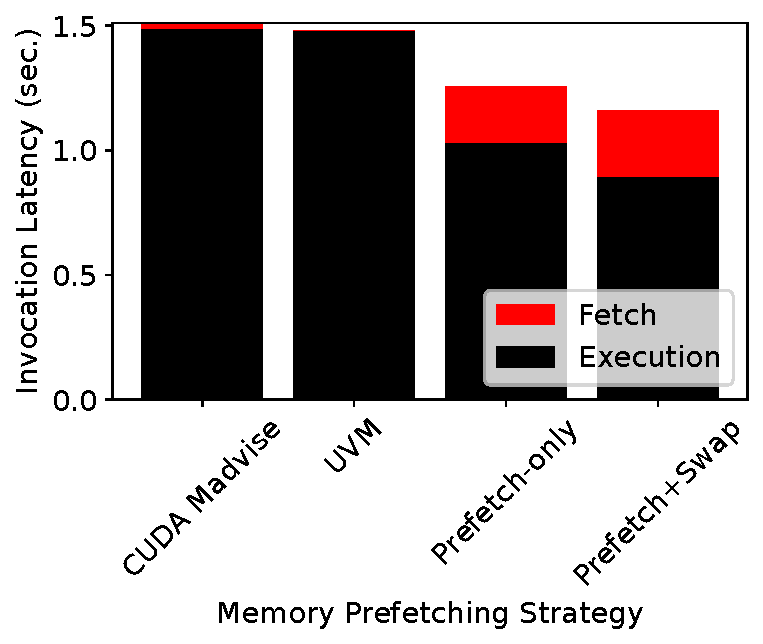
\includegraphics[width=0.45\textwidth]{../graphs/mem-move/f16-i20-driver-mps-move.pdf}
  \vspace*{\captionspace}
  \caption{More intelligent memory management improves execution latency. 
    \texttt{Prefetch To} moves memory on-device before a function container executes.
    \texttt{Prefetch} additionally moves it off again when the container will be idle.}
    \label{fig:mem-prefetch}
    \vspace{\myfigspace}
% Fetch Strat, Exec Time, Fetch Time, Total Time
% Madvise 1.4893044978380203 0.021360369771718932 1.5106648676097392
% None 1.4704825393855572 1.2621283531188965e-06 1.4704838015139103
% Prefetch To 0.830518102645874 0.4062889523804188 1.2368070550262928
% Prefetch 0.7852441824972629 0.22023404985666276 1.0054782323539257
\end{figure}


\mhead{Interception Overhead}
We intercept driver calls and replacing physical memory allocations with UVM to enable memory management, but this change comes with a price.
To determine the impact, we run each function 10 times, with and without our driver shim enabled, tracking their latency.
We never adjust where the function's memory is, so any overhead will be caused by interceptions and usage of UVM allocations.
Figure~\ref{fig:shim-overhead} collates a variety of different function types and how they were affected.
Most functions see zero added execution time from the shift to UVM, our interception being undetectable.
The rest see single-digit percentage increases, with \funcname{Srad} standing out with a 30\% overhead in execution time under the shim.
These results are in line with Nvidia's own reporting on the performance change when migrating applications to UVM~\cite{nvidia-uvm}.
With our driver having such little impact, it is ideal for enabling a warm container pool of GPU containers and moving function memory off device when idle.

\begin{figure}
  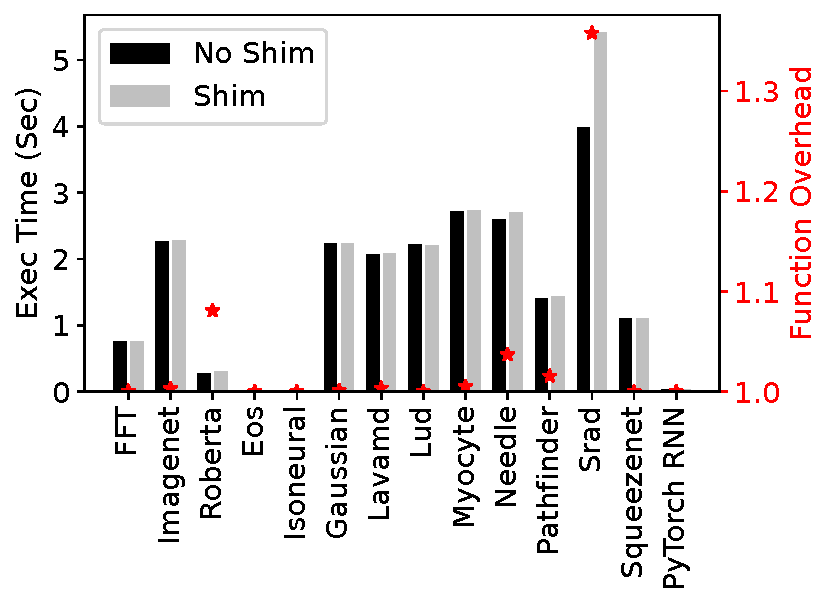
\includegraphics[width=0.45\textwidth]{../graphs/driver-compare/8-exec_time.pdf}
  \vspace*{\captionspace}
  \caption{Functions see little to no impact from our interception and substitution of allocation calls.
          This matches performance promised by Nvidia for UVM applications.}
    \label{fig:shim-overhead}
    \vspace{\myfigspace}
\end{figure}

\subsection{Queuing Knobs}
\label{sec:queue-knobs}

Knowing we can efficiently manipulate GPU memory, we move to testing our queuing policies built on top of them.
Our queue design allows for a number of hyperparameters that are either fixed by configuration or dynamic at runtime.
Here we explore the effects of each knob in isolation to see their effect on performance.

Each experiment is run with the same trace composed of 18 functions, run for 10 minutes, have roughly 2 invocations per second, and presented results are the average of 5  repeated runs.
Function were randomly chosen from Azure trace in the same manner as previous works~\cite{fuerst2023iluvatar,faaslb-hpdc22}, and the trace generated by randomly sampling from an eCDF computed from the Azure data.
To map a function name to actual GPU code, we select the closest matching execution duration from Table~\ref{tab:gpu-cpu} that doesn't exceed that time.

\mhead{Container Pool}
% Functions running warm is vital for low latency in serverless systems which, and our UVM shim enables maintaining a warm pool of GPU containers.
To show the effectiveness of both \QName's sticky dispatching and having a container warm pool are at decreasing cold hits, we increase the number of functions to 65 while keeping the invocations per second similar.
Experiment duration is increased to one hour to prevent first-time invocations of functions, which will always be cold starts, from dominating the results.
% To show how cold hits decrease as the warm pool is enabled we increase the number of functions to 65 and the duration to one hour while keeping the invocations per second similar.
% The high number of functions will stress the need for having available containers 
The high number of functions stresses the need for having a warm pool, as is clear from the results in Figure~\ref{fig:container-pool-cold-hits}.
A simple FCFS queuing policy that has no warm pool (e.g. pool size of 1) sees colossal 90\% cold hit rate.
%  caused by both the lack of warm pool and inability to reorder enqueued invocations so that they may run warm.
% Looking at the blue line, with no pool, (e.g. a pool size of 1), 10\% of invocations run cold, which cause a knock-on effect of higher latencies for both the invocation run cold and those waiting in queue.
Comparatively with the same lack of pool, \QName~without concurrency, represented by the blue line, only has 10\% of invocations run cold.
%  kept low entirely by its locality measures.
\QName's improvement comes from its locality and overrun techniques, as FCFS cannot reorder invocations and must frequently evict container to run the next item.
% Note that \QName~doesn't intentionally optimize for running a function in a warm container, but this emerges due to its overrun and throttling policies.
% This number are low to start thanks to the locality measures in \QName, comparatively, a FCFS Naïve queuing policy sees a much higher 90\% cold hit rate.
When the pool is increased to 32 containers, only 2\% of \QName~invocations are cold, which continue to decline with higher sizes.
FCFS also benefits from the warm pool, with both policies having equal cold hits when the pool size is maximized.

When we increase concurrency (\D), two scenarios come up: either different functions run concurrently with each other, or a function runs concurrently with itself.
The latter causes higher cold starts as we need one container per dispatched invocation of the same function.
Green and orange lines in Figure~\ref{fig:container-pool-cold-hits} show the impact of \D~on cold starts.
% High numbers equivalent to the no-pool case appear, and are again mitigated by the larger pool size.
Cold hits are higher with concurrency as expected, but are mitigated once the warm pool size grows to 32.

\begin{figure}
  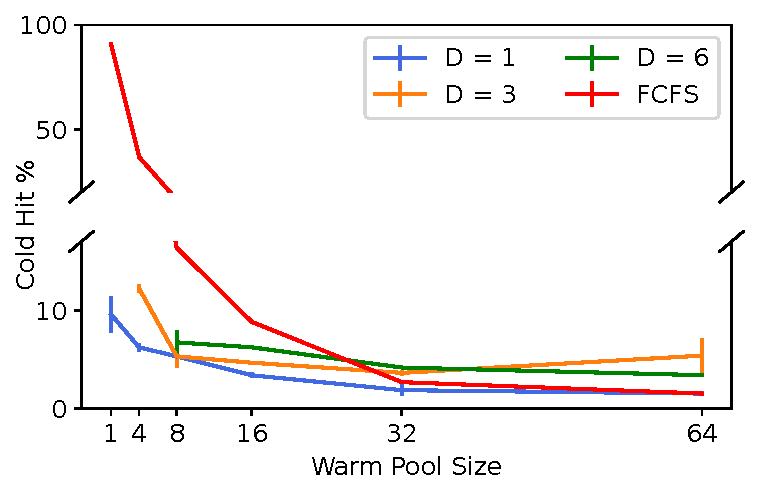
\includegraphics[width=0.45\textwidth]{../graphs/container_pool/big-60min/65/cold_hits.pdf}
  \vspace*{\captionspace}
  \caption{\QName~greatly reduces cold hits compared to FCFS, and is improved with a large container pool size. 
          More cold hits are also caused when \D~(concurrency) is raised, needing private containers to serve concurrent invocations.}
    \label{fig:container-pool-cold-hits}
    \vspace{-0.4cm}
\end{figure}

\mhead{Unfairness}
The limited resources on GPUs encourages us to prefer running a function several times because its resources are already on-device.
Adjusting the maximum overrun \T~to find the ideal balance point between fairness and stickiness is important.
% Figure~\ref{fig:unfairness-queue} shows how performance can be improved by allowing some unfairness by adjusting \T, the maximum allowed overrun of a flow.
% Figure~\ref{fig:unfairness-queue} are the average of time spent in the queue, with each function's queue time being normalized by their fraction of invocations in the trace.
Figure~\ref{fig:unfairness-queue} compares the average invocation latency as we increase \T.
Using a fixed increment to \VT~(i.e. 1.0 in Figure~\ref{fig:unfairness-queue}) is a simple solution and forces functions' to have an equal \emph{number} of invocations.
Such a policy ignores functions' variable execution times, favoring those with long execution times, and as seen in many other scheduling domains leads to unfairness and poor performance.
When $\T \le 1$, each flow is immediately throttled after a completed dispatch, forcing it to lose on-device locality, and has a terrible impact on latency.
% Larger \T, up to 10, improve latency by up to 25\%, a notable benefit provided by locality,
As \T~increases, latency is improved by up to 25\% at $\T == 10$, locality causing invocations to complete faster and increasing flows drainage.

The service average by which we increase a flow's \VT~has a significant impact queuing.
Using function execution time (Wall Time) as the service average changes \VT~to represent \emph{time} on device per-function.
Execution time is highly variable in FaaS unlike MQFQ's disk I/O domain, and ignoring it can lead to unfairness.
% Small yet popular functions are frequent in FaaS, favoring them shows when the best performance.
With $\T \approx 5$, latency is 70\% better than with immediate throttling, and 60\% better at this point over the fixed service average.
When \T~becomes too large, device time is hogged by specific flows, unfairness becomes extreme, and we see worse invocation latency.
% Favoring short functions will be allowed to run several times before being replaced with a long one.
% A flow with a long-running function 

\begin{figure}
  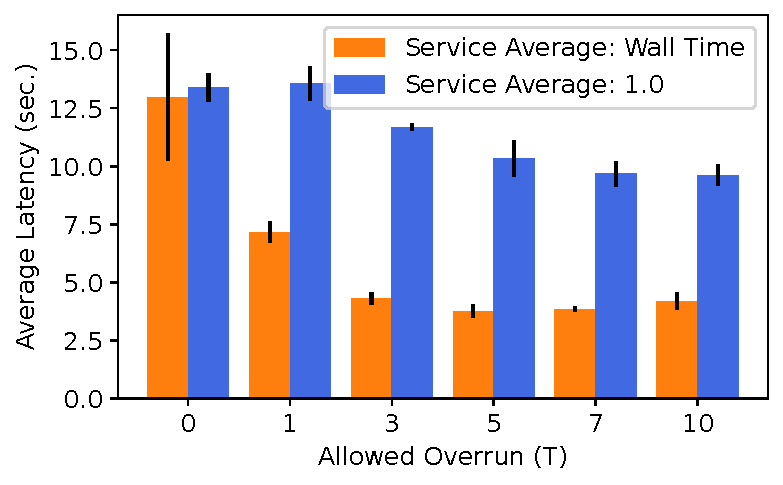
\includegraphics[width=0.47\textwidth]{../graphs/unfairness/25.7/e2e_sec.pdf}
  \vspace*{\captionspace}
  \caption{Adjusting \T~allows flows to overrun one another, increasing data locality and therefore performance.
  The performance changes when a function's GPU wall time is used to change \VT, or the increment is fixed.}
    \label{fig:unfairness-queue}
    \vspace{-0.4cm}
\end{figure}

\mhead{Active Flow TTL}
A larger \T~is not the only way tool design has to favor locality, we can also keep a flow \emph{active} even while empty.
Empty flows remain active until a TTL expires, then they're made inactive and have resources moved off device.
Figure~\ref{fig:flow-ttl} shows the improvement to both execution time as compared to ideal warm performance (improved by local resources), and latency (additionally improved by priority dispatching) as the TLL grows.
Setting any global TTL (the solid line), at even a small 0.1 seconds, improves latency and overhead by 25\% and 50\% respectively.
% Latency sees a 25\% improvement and execution time over 50\%, from \emph{any} TTL policy, and 
Increasing the TTL to up to 4 seconds sees significant, but diminishing, returns.

% A large 4 second time can reduce latency by 35\% and execution time by 40\%.
We can also base the TLL on each function's inter-arrival-time (IAT), rather than have a global fixed time.
This method sets the TTL for each flow to the IAT multiplied by the value on the X axis, plotted as the dashed line.
Switching generally performs better, and performs best when $TTL = IAT \times 1.5$, reducing invocation latency by 40\% over no-TTL.
These results fit the heterogeneous and bursty nature of FaaS functions with varied IATs.
Even popular functions with low IAT can have idle periods, and keeping their resources warm for short periods allows fast handling when they re-appear.
Setting the TTL too high at $IAT \times 3$ prevents them from transitioning to inactive, leaving their \VT~artificially low, jumping them unfairly ahead in the queue.

\begin{figure}
  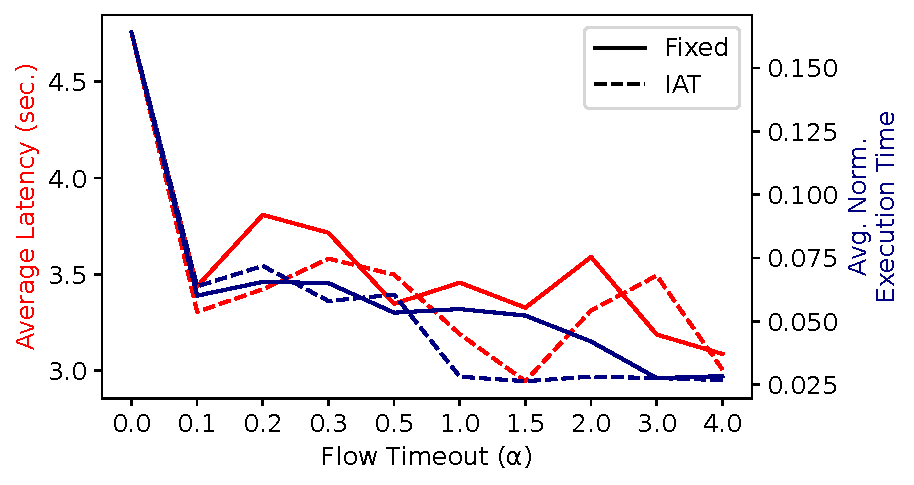
\includegraphics[width=0.45\textwidth]{../graphs/ttl/25.8/mqfq-ttl-compare.pdf}
  \vspace*{\captionspace}
  \caption{Enabling a time-to-live for flows prevents them from becoming inactive, to keep resources warm on-device. 
    This improves both latency and on-device execution time for functions.
    Note the non-linear scale on the X axis.}
    \label{fig:flow-ttl}
  \vspace{-0.5cm}
\end{figure}


\mhead{Concurrency}
Running concurrent invocations is vital to achieving high GPU utilization, and by improving invocation throughput aids user latency.
% We monitor the utilization of GPUs every 200 ms, as well as when functions launch and complete.
Figure~\ref{fig:concur-exec-overhead} examines the effect on execution overhead as the concurrency \D~is changed and is made dynamic.
When \D~is fixed, the gray line, overhead is directly correlated with \D, added up to 2x overhead from GPU contention.
The remaining lines represent the GPU utilization percentage at which we dynamically adjust \D~but have a fixed maximum (\Dmax), represented by the X axis value.
% In the dynamic case, when the compute utilization is below 95\%, we increase \D~and dispatch a new invocation.
% \D~is capped by a maximum configuration setting to prevent runaway dispatching that can occur during time in between active function's kernel launches.
All see a small increase in overhead when $\Dmax==2$, equal between all values.
% A low percentage such as 50\% has stable overhead close to that of when $\D==1$, but at the expense of high queuing time due to lack of dispatches.
Higher \Dmax~sees them separate but reach a plateau of maximum overhead, as the GPU manager limits \D~as it detects high device contention.

% Execution time isn't the only metric impacted, 
Latency for invocations also changes as \D~is adjusted, throughput at the expense of individual invocation overheads.
Latency in Figure~\ref{fig:concur-e2e} is decreased across the board when $\Dmax==2$, and nearly 20\% better than baseline when utilization monitoring is at 80\%.
This trend does not continue, caused by queuing at the conservative level of 50\% and encroaching execution overhead at higher levels.
The scalability of \D~hinges on a variety of factors: function workload composition, device compute capability, and device memory size.
Larger devices can support more functions, but this can be offset by an equally expensive function to run.

\begin{figure}
  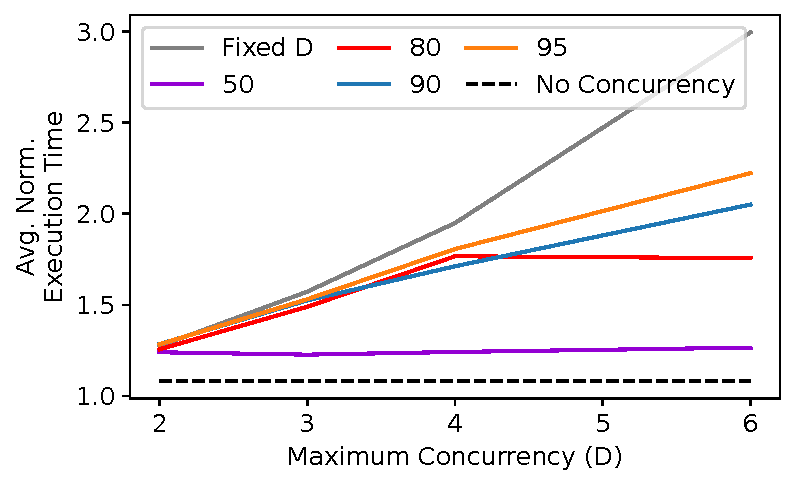
\includegraphics[width=0.45\textwidth]{../graphs/concurrency/25.7/paper_exec_overhead.pdf}
  \vspace*{\captionspace}
  \caption{Execution overhead grows as concurrency is increased.
  The gray line uses a fixed device concurrency, and the remaining lines represent the GPU utilization below which we allow a new dispatch.}
    \label{fig:concur-exec-overhead}
    \vspace{\myfigspace}
\end{figure}
\begin{figure}
  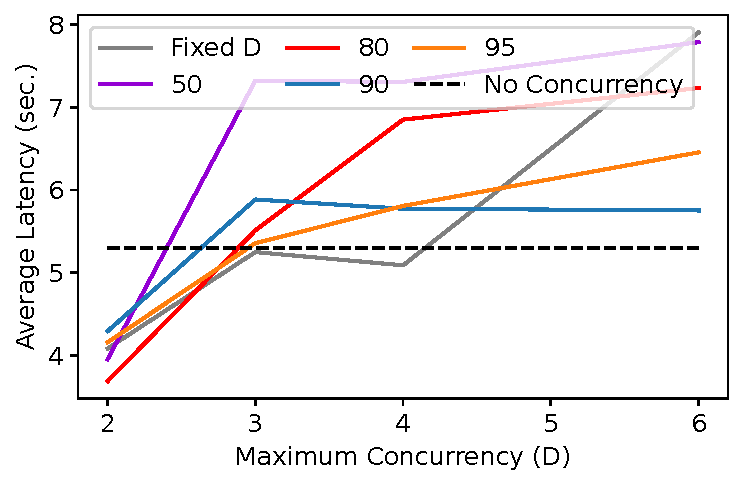
\includegraphics[width=0.45\textwidth]{../graphs/concurrency/25.7/paper_e2e_sec.pdf}
  \vspace*{\captionspace}
  \caption{Latency for invocations is affected by concurrency.
  Increasing \D~when utilization is low improves latency, but if the threshold is too high, significant queuing delays occur.}
  \label{fig:concur-e2e}
  \vspace{-0.5cm}
\end{figure}
\begin{comment}
\mhead{Flow Weights}

Flow weights comparison - Figure~\ref{fig:flow-weights}

\begin{figure}
  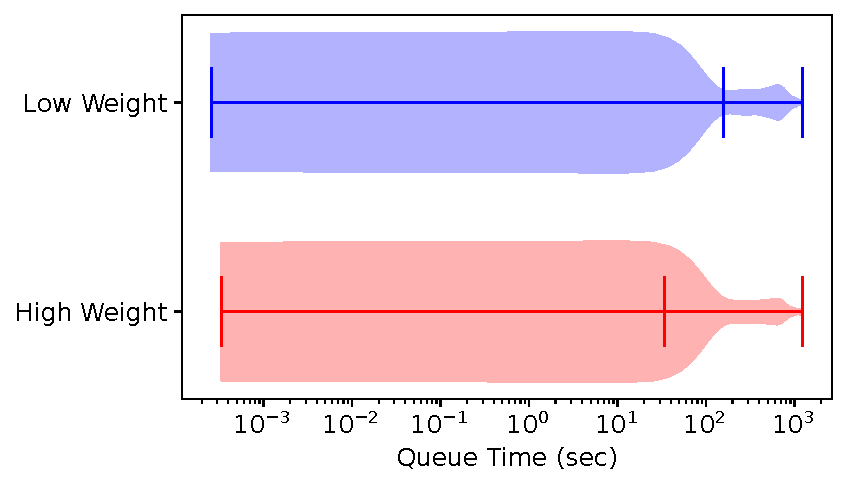
\includegraphics[width=0.45\textwidth]{../graphs/weights/13.9/weight_box_log.pdf}
  \caption{Flow weights can influence queueing time and latency.}
    \label{fig:flow-weights}
\end{figure}
\end{comment}

\subsection{\QName~Performance}
\label{sec:queue-perf}

Now that we've shown how \QName's performance is affected by hyperparameters, we look at the optimal configuration and compare to other policies.
We show three alternative policies as comparison, \naive, \fcfs, and \batch.
\naive~dispatches in a first-come-first-serve order and has no container pool, \fcfs~uses our warm pool and shim to move function memory on-device before executing, and move it back off after each invocation has completed.
% and a \texttt{Batch} policy that separates flows and executes everything in the flow with the
Thirdly, a variant we call \batch~also inserts invocations into per-function flows, and on dispatch empties the entire \emph{flow} containing the oldest \emph{item} to execute all removed items serially, but prevents new items from tagging along.
% The latter two have been enhanced to use our shim to move function memory on-device before executing, and move it back off after invocation completion.
It also uses the warm pool and memory movement, only does this after the completion of an entire batch.

Starting with the worst-performing policy in Figure~\ref{fig:queue-e2e}, \naive~has extreme wait times caused by frequent cold starts caused by the lack of warm pool as we saw in Fig.~\ref{fig:container-pool-cold-hits}.
Adding the pool and memory management in \fcfs~gives over two orders of magnitude improvement in latency, without increasing the concurrency.
\QName~outperforms \fcfs~by 3x with a 3.9 vs 13-second average respective latency thanks to its locality favoring overrun mechanism.
% , and 20\% better than \batch~because it doesn't throttle functions that hog GPU time well.
Increasing \D~improves \QName~latency by a further 15\% and actually makes \batch~have equal performance.
This is caused by errant lucky items at the end of batches jumping ahead in the queue, in violation of fairness principles.
When \D~is set too high, the device cannot handle the higher concurrency, and all policies suffer degradation from compute contention.

\begin{figure}
  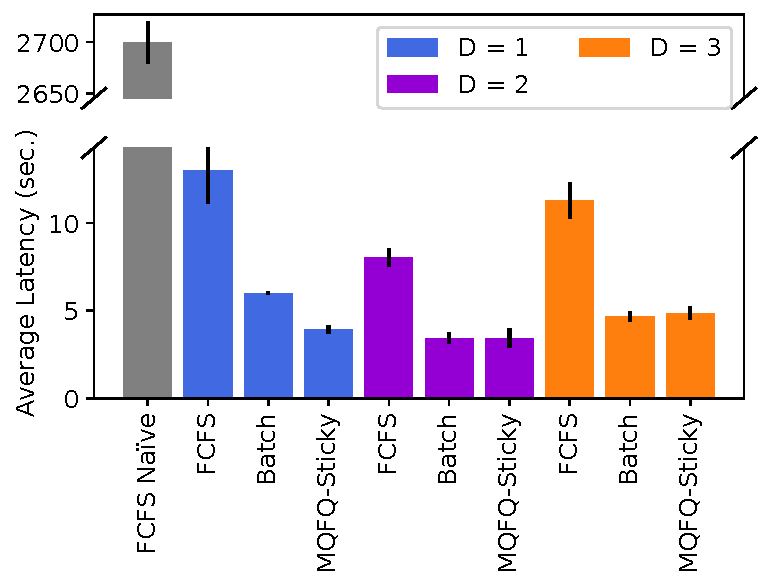
\includegraphics[width=0.45\textwidth]{../graphs/q_compare/25.7/20/paper_e2e_sec.pdf}
  \vspace*{\captionspace}
  \caption{Latency of various queue policies compared.}
  \label{fig:queue-e2e}
  \vspace{\myfigspace}
\end{figure}

% 25.7 20
% ['FCFS', 'Batch', 'MQFQ-Sticky', 'FCFS', 'Batch', 'MQFQ-Sticky', 'FCFS', 'Batch', 'MQFQ-Sticky']
% [12.995100928987991, 6.008403172041167, 3.9393128576329333, 8.030896226415095, 3.4407989024013723, 3.4336443728987986, 11.269908295197256, 4.6764212401266105, 4.865312288850772]
% 25.7 0.3
% ['FCFS', 'Batch', 'MQFQ-Sticky', 'FCFS', 'Batch', 'MQFQ-Sticky', 'FCFS', 'Batch', 'MQFQ-Sticky']
% [12.995100928987991, 6.008403172041167, 4.167263608404803, 8.030896226415095, 3.4407989024013723, 3.8459053233276164, 11.269908295197256, 4.6764212401266105, 4.868836489708405]
% 25.7 3
% ['FCFS', 'Batch', 'MQFQ-Sticky', 'FCFS', 'Batch', 'MQFQ-Sticky', 'FCFS', 'Batch', 'MQFQ-Sticky']
% [12.995100928987991, 6.008403172041167, 4.854454444082333, 8.030896226415095, 3.4407989024013723, 3.841766863464837, 11.269908295197256, 4.6764212401266105, 4.819323267753003]

\mhead{\QName~Fairness}
\todo{Text for Figure~\ref{fig:queue-fairness}}

\begin{figure}
  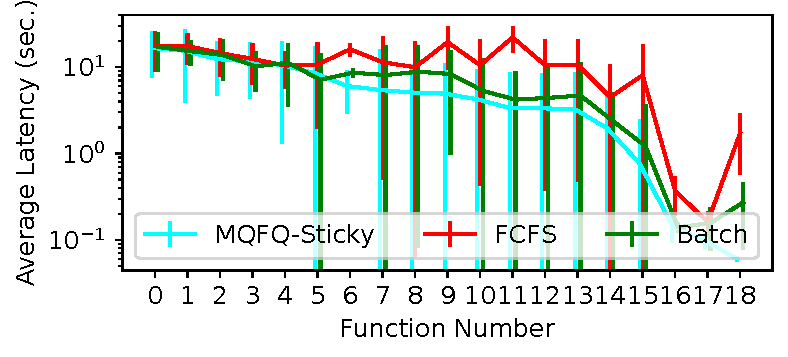
\includegraphics[width=0.45\textwidth]{../graphs/q_compare/25.7/20/paper_fairness_squish.pdf}
  \vspace*{\captionspace}
  \caption{Per-function latency comparison between FCFS and \QName.}
  \label{fig:queue-fairness}
  \vspace{\myfigspace}
\end{figure}

\begin{comment}
\begin{figure}
  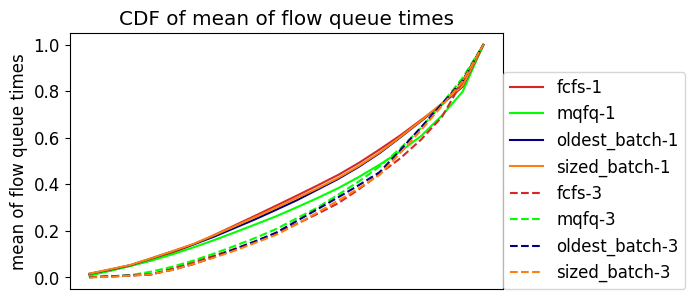
\includegraphics[width=0.45\textwidth]{../graphs/q_compare/25.7/mean_flow_fairness.png}
  \caption{Fairness of various queue policies compared.}
    \label{fig:queue-fairness}
\end{figure}

\mhead{GPU Utilization}
\end{comment}

\mhead{Multiple GPUs}
Our system easily scales to orchestrating and dispatching across multiple GPUs.
We run the same trace as in previous experiments and show the comparison in Figure~\ref{fig:multi-gpu} after we add a second, identical, GPU to our hardware.
% In Figure~\ref{fig:multi-gpu} we show how it adapts to running the same trace on systems with one and two identical GPUs.
Two GPUs not only allows us to run $\D\times2$ invocations, but also do on-the-fly load balancing between them to avoid compute contention with higher \D.
% and therefore expect a corresponding 2x performance improvement.
As a baseline, the multi-GPU blue dashed line has 60\% lower latency without device concurrency.
Scaling \D~to 6, we see reductions in latency up to \emph{87\%} -- whereas the single device is quickly overloaded and has worse overall performance.
% This balancing boosts latency reduction to \emph{87\%} when \D~is very high
% , much better than our expected linear speedup.
Execution overhead in red increases dramatically with \D~when only one GPU is available, in the worst case a nearly 6x increase.
% With higher \D, our dispatches also load balance between the two devices, something not possible in the solitary device case.
However, with two GPUs in the red dashed line, once $\D \ge 2$ the load balancing mitigation lowers overhead by 45\%, and a maximum of 66\%.
Reduction of this overhead is a significant contributor to lower latencies as well.
% The ability to choose devices results in a 70\% reduction in execution overhead, entirely from mitigating compute overloading.


% e2e
% [4.663137860034904, 3.607658436985101, 4.575037657122783, 4.991578333097969, 5.386245616200919, 5.212470496279234]
% [1.9581354786418401, 1.0854709685368538, 0.8082406824696803, 0.7523517956355057, 0.7496512471943295, 0.677325266114725]
% [0.58008201 0.69912036 0.82333682 0.84927577 0.86082119 0.87005677]
% exec
% [0.07375773205618323, 0.27254631424617926, 0.4598690614061698, 0.8230379144178025, 1.0323527250435014, 1.154964442968281]
% [0.08146243318283061, 0.14722147302861147, 0.2398143374961277, 0.2358641959639591, 0.341338564858076, 0.3858309500976596]
% [-0.10445957  0.45982952  0.47851604  0.71342244  0.66935859  0.66593695]

\begin{figure}
  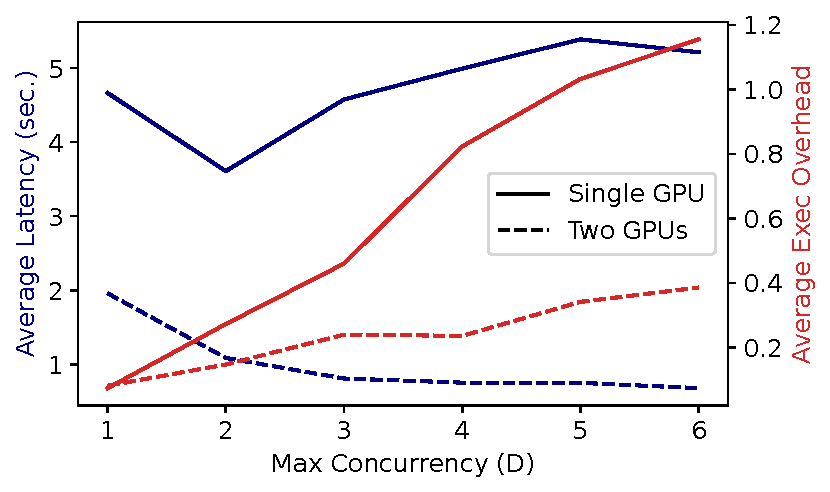
\includegraphics[width=0.45\textwidth]{../graphs/multi-gpu/25.7/concurr_scale.pdf}
  \vspace*{\captionspace}
  \caption{Dispatching to multiple GPUs greatly improves latency and execution overhead compared to a single GPU.
  }
  % Latency results are in dark blue, and execution overhead in red. 
  % The solid lines of the single GPU case are much worse than when scaling to two GPUs in the dashed line.
  % }
  \label{fig:multi-gpu}
  \vspace{-0.65cm}
\end{figure}

\mhead{Dynamic Compute Selection}

% \todo{Figure~\ref{fig:poly} text}
Just because an item can run on GPU, doesn't mean it has to.
We took a third of the functions in our trace, those having a speedup from running on GPU of 3x or less, and configured them to only run on CPU.
These functions may have longer execution times, but avoid queuing for the GPU and run immediately on the system's plentiful CPU.
The effect on system performance from this shift can be seen in Figure~\ref{fig:poly}.
Average latency drops from 3.4 to 0.99 seconds, a 72\% decrease.
This dramatic change isn't just from a few functions avoiding the queue, their removal also reduces pressure on GPU resources.
\QName~can more easily maintain locality for the smaller selection of functions and reduce overhead they see.
Removing the need to context-switch for certain functions that see little benefit from acceleration can help both categories of function.

\begin{figure}
  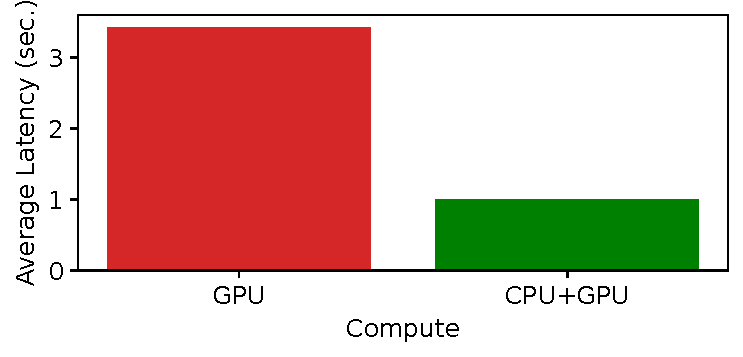
\includegraphics[width=0.45\textwidth]{../graphs/polymorphic/25.7/compute_compare_squish_focused.pdf}
  \vspace*{\captionspace}
  \caption{Dynamically selecting what compute a function runs on can reduce GPU queuing and improve global latency.}
  \label{fig:poly}
  \vspace{-0.3cm}
\end{figure}

% CPU 2.030147525728988
% GPU 3.4336443728988
% Two GPUs 1.0899518145507185
% CPU/GPU 0.9972267068610635